%%
%% pytorch-neural-doodle/docs/content/chapters/03_results.tex
%%
%% Created by Paul Warkentin <paul@warkentin.email> on 21/08/2018.
%% Updated by Bastian Boll <mail@bbboll.com> on 07/10/2018.
%%

\clearpage
\section{Results}
\label{section:results}

\textbf{by Paul Warkentin} \\

We reproduced the results of \cite{doodles2016} by implementing the described algorithms on top of pytorch\footnote{The code for this implementation is publicly available at \url{https://github.com/paulwarkentin/pytorch-neural-doodle}. See the Readme for additional information.}. It is to be noted that style transfer using the approaches presented in the present work has at its heart an optimization procedure which is very demanding in terms of GPU memory and compute capability. The high memory requirements stem from the need to save and evaluate image patches. Fundamentally, the procedure takes time, because computing a gradient of the loss function requires a backward pass through the VGG network. Figure \ref{fig::phases} displays the progress of an L-BFGS optimizer for the generation of a stylized image.

\begin{figure}
	\begin{subfigure}[t]{0.23\textwidth}
		\centering
		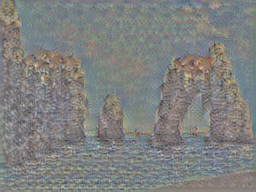
\includegraphics[width=3.5cm]{phases/output-50.png}
	\end{subfigure}%\hspace{5mm}
	~
	\begin{subfigure}[t]{0.23\textwidth}
		\centering
		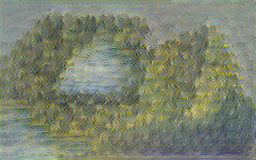
\includegraphics[width=3.5cm]{phases/output-200.png}
	\end{subfigure}%\hspace{5mm}
	~
	\begin{subfigure}[t]{0.23\textwidth}
		\centering
		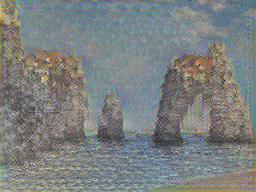
\includegraphics[width=3.5cm]{phases/output-400.png}
	\end{subfigure}
	~
	\begin{subfigure}[t]{0.23\textwidth}
		\centering
		\includegraphics[width=3.5cm]{phases/result.png}
	\end{subfigure}
	
	\caption[]{Progress of an L-BFGS optimizer for the generation of a stylized image. Iteration count from left to right: 50, 200, 400, 500.}
	\label{fig::phases}
\end{figure}

When using modern hardware (at the time of writing e.g. an NVIDIA GTX 1080 Ti) with sufficient GPU memory, generating a single image requires computation time on the order of minutes. The samples in figure \ref{fig::nocontent} were generated in approximately eight minutes each. 

In addition to the examples presented in \cite{doodles2016}, we chose another content and style image and authored a segmentation. The results\footnote{The original artwork for the style image is by Mia Bergeron \url{http://www.miabergeron.com}.} are presented in figure \ref{fig::freddie}.

\begin{figure}
	\begin{subfigure}[t]{0.18\textwidth}
		\centering
		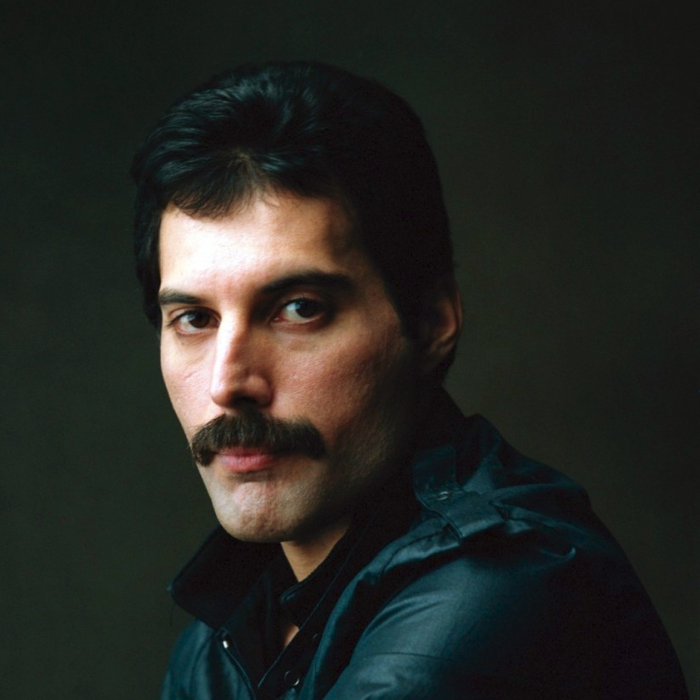
\includegraphics[width=2.9cm]{freddie/freddie.png}
	\end{subfigure}%\hspace{5mm}
	~
	\begin{subfigure}[t]{0.18\textwidth}
		\centering
		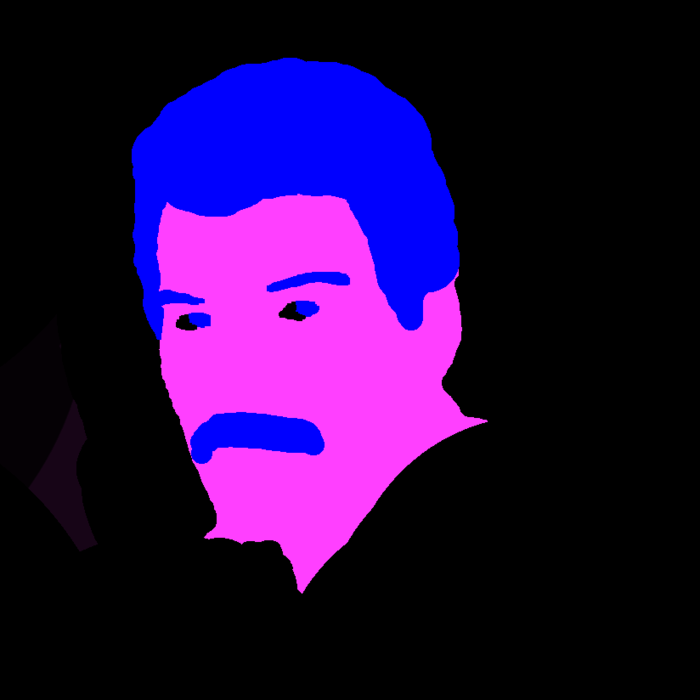
\includegraphics[width=2.9cm]{freddie/freddie_map.png}
	\end{subfigure}%\hspace{5mm}
	~
	\begin{subfigure}[t]{0.18\textwidth}
		\centering
		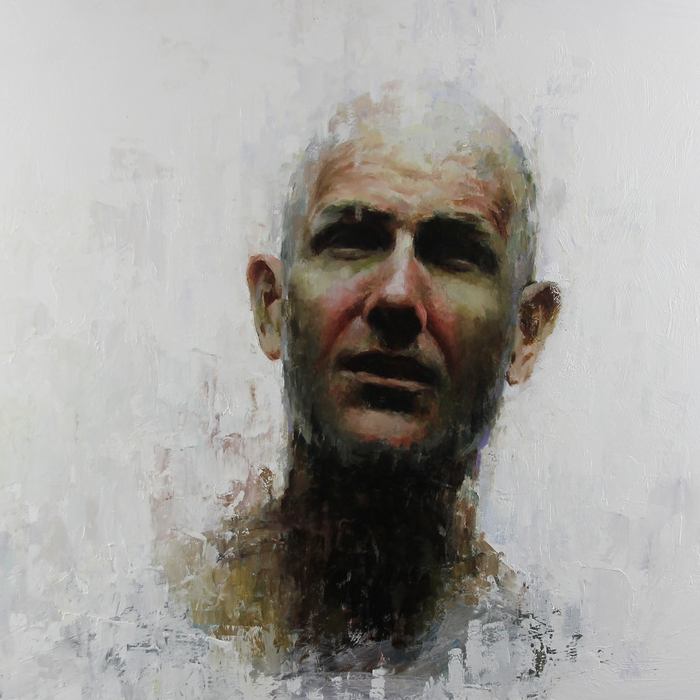
\includegraphics[width=2.9cm]{freddie/bergeron.png}
	\end{subfigure}
	~
	\begin{subfigure}[t]{0.18\textwidth}
		\centering
		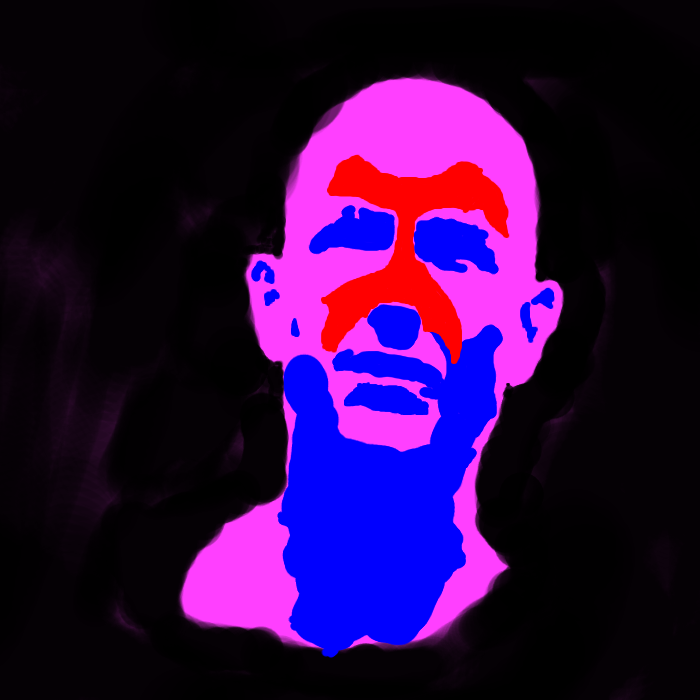
\includegraphics[width=2.9cm]{freddie/bergeron_map.png}
	\end{subfigure}
	~
	\begin{subfigure}[t]{0.18\textwidth}
		\centering
		\includegraphics[width=2.9cm]{freddie/result.png}
	\end{subfigure}
	
	\caption[]{Application of full artistic style transfer. From left to right: Content image, content segmentation, style image, style segmentation, generated result.}
	\label{fig::freddie}
\end{figure}